\section{Results}
\label{sec:nt-results}

\subsection{The naming turn and its decomposition}
\label{sec:nt-turn}

\paragraph{Shape.}
\NAME{} titles were 8.9\% of ICLR submissions in 2017, 20.3\% in 2023 and 40.5\% in 2026; compound titles rose from 19.3\% to 59.9\% (Table~\ref{tab:nt-corpus}, Figure~\ref{fig:nt-turn}a). % features/fig_name_share_by_year.csv
On the log-odds scale, on which diffusion is usually judged \citep{bass1969new}, the share has followed a steady logistic path since 2017: the 2017--23 pre-trend is OR 1.125 per year (odds $+12.5\%$ a year), and this trend alone projects 35.0\% for 2026. Deviations from it are $+1.5$\pp{} \ci{-0.7}{3.8} in 2024, $+2.7$\pp{} \ci{-0.5}{5.9} in 2025 and $+5.5$\pp{} \ci{1.5}{9.5} in 2026. The year-level log-odds slope change at 2024 is OR 1.096 \ci{0.990}{1.214} (one-sided $p=0.035$; Holm 0.071; paper level 1.098 \ci{1.044}{1.154}). A constant log-odds slope is already convex on the probability scale, where the slope change is $+2.8$\pp{} per year \ci{1.3}{4.4}; we report this only as a secondary description. The camera-ready-free pool tracks all submissions (40.3\% in 2026; year-level slope change 1.121 \ci{1.019}{1.232}), so the rise is not a camera-ready artefact. The rise is also present outside LLM topics (19.5\% to 36.0\% between 2023 and 2026), but there the year-level slope change, 1.108 \ci{0.986}{1.245}, includes 1. Compound titles show a larger paper-level slope change, 1.231 \ci{1.176}{1.289} (Table~\ref{tab:acceleration}).

\paragraph{Timing and the 2026 cohort.}
The acceleration is not a dated break. The pre-specified sup-LR scan selects 2023, not 2024, and a 2023 break, a 2024 break, a 2024 kink and a quadratic trend fit about equally well. 2026 is the year of a new desk-rejection regime and has 15,412 of the 43,482 papers. \textbf{The acceleration depends on 2026; the carrier, slot and filter results do not} (Table~\ref{tab:nt-2026}). Nothing in this design ties the timing to ChatGPT.

\begin{table}[t]
\centering
\scriptsize
\setlength{\tabcolsep}{2pt}
\caption{Which results depend on 2026. 95\% CIs (90\% for the NAME filter gain). Sources: \texttt{d1\_break}, \texttt{d2\_carriers}, \texttt{d3\_register}, \texttt{d4\_filter} RESULTS.md.}
\label{tab:nt-2026}
\begin{tabular}{@{}p{2.5cm}ll@{}}
\toprule
Result & All years & Without 2026 \\
\midrule
NAME slope change, year level (OR) & 1.096 \ci{0.990}{1.214} & 1.046 \ci{0.807}{1.355} \\
Unexplained-drift acceleration (pp) & $+1.35$ \ci{0.03}{2.71} & $+1.15$ \ci{-0.63}{2.96} \\
Stayer ratio, last position$^a$ & 0.995 \ci{0.943}{1.050} & 1.003 \ci{0.918}{1.095} \\
First $-$ last stayer ratio$^a$ & $-0.470$ \ci{-0.602}{-0.359} & $-0.474$ \ci{-0.670}{-0.276} \\
Pooled slot OR at 2024 & 2.18 \ci{1.41}{3.38} & 2.27 \ci{1.36}{3.80} \\
NAME filter gain, accepted/all & 1.021 \ci{1.001}{1.041} & 1.037 \ci{1.008}{1.068} \\
\bottomrule
\multicolumn{3}{@{}p{7.4cm}@{}}{\scriptsize $^a$ Without 2026: E $=$ 2021--22, L $=$ 2024--25. 2026 composition by affiliation or country cannot be measured from the export.}
\end{tabular}
\end{table}

\begin{figure*}[t]
\centering
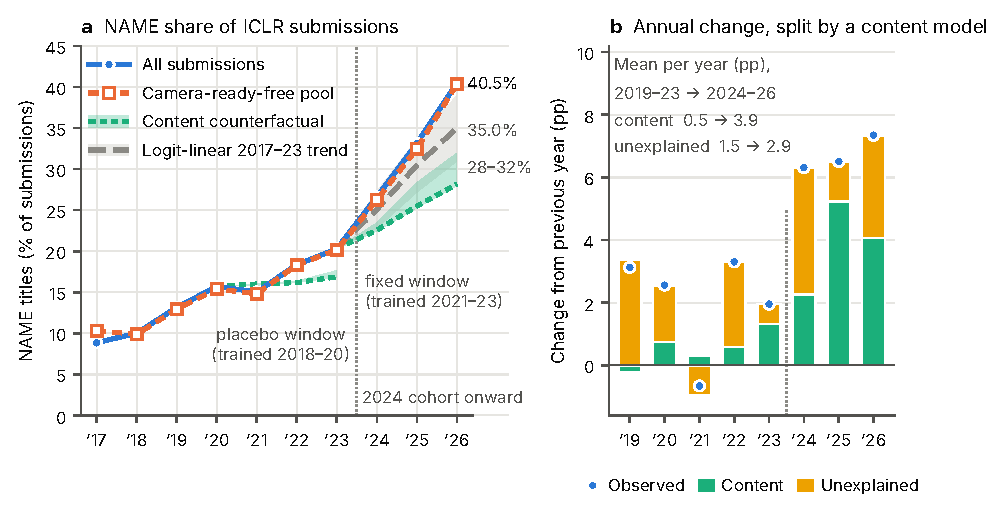
\includegraphics[width=0.92\textwidth]{fig1_naming_turn.pdf}
\caption{\textbf{The naming turn.} (a) \NAME{} share of ICLR submissions (discovery split), for all submissions and the camera-ready-free pool, against the logit-linear 2017--23 trend (dashed; band from the year-deviation CIs) and name-masked content counterfactuals (dotted: masked TF-IDF, fixed window; ribbon: range over the three masked representations in the fixed and rolling designs; the placebo window trained on 2018--20 already under-predicts 2021--23). The content counterfactuals (28--32\% in 2026) lie below the trend (35.0\%). (b) Annual change split into the part predicted by a rolling name-masked content model and the unexplained part. Mean content steps rose from 0.5 to 3.9\pp{} per year and unexplained steps from 1.5 to 2.9\pp{} per year (2019--23 $\rightarrow$ 2024--26); the difference in unexplained steps, $+1.35$\pp, has a two-stage year-level 95\% CI of \ci{0.03}{2.71}.}
\label{fig:nt-turn}
\end{figure*}

\paragraph{Content.}
How much of the 2023$\rightarrow$26 rise does the content of the papers track? Name-masked content models give 0.39 \ci{0.35}{0.43} (masked TF-IDF) and 0.49 \ci{0.44}{0.54} (masked bge) in a fixed window trained on 2021--23, and 0.57 \ci{0.53}{0.62} and 0.58 \ci{0.53}{0.63} in a rolling one-step design. Across specifications (training-year effects, slope recalibration) the share ranges from \textbf{0.37 to 0.65} (Table~\ref{tab:content}). The content counterfactuals reach 28--32\% in 2026, below the naive 2017--23 trend (35.0\%): part of what the trend ``predicts'' is not carried by content. The one \emph{additive} split is the fixed-window Shapley decomposition: content 0.34, composition 0.09 and unexplained 0.57 (refit bootstrap \ci{0.48}{0.67}) (Figure~\ref{fig:nt-decomp}a). The other estimators come from different designs and cannot be summed. The content signal is dominated by LLM-era topic words (\emph{reasoning, generation, benchmark, evaluation}), so ``content'' includes the move into LLM topics, the channel through which the writing tool also operates.

\paragraph{Branding runs ahead of content in new topics.}
The pre-specified new-topic placebo fails in every window. In topic clusters whose share grew at least threefold, observed \NAME{} exceeds the content prediction by 15.8\pp{} against 7.7\pp{} elsewhere (year-averaged absolute residuals, fixed 2024--26 window), a gap difference of 8.0\pp{} \ci{6.8}{9.2}. The pattern already appears in the pre-LLM placebo window (3.6\pp{} \ci{1.0}{6.2}). Either naming is a property of new artefact-producing topics that bag-of-words content misses, so content shares are understated, or the fashion spreads fastest in hot topics.

\paragraph{Composition and detectable LLM drafting.}
Reweighting 2024--26 papers to the 2023 distribution of team size $\times$ new-key share $\times$ LLM topic accounts for 0.29, 0.32 and 0.26 of the rise in 2024, 2025 and 2026 (DFL), but only 0.09 net of content (Shapley). Mean declared author-list size rose from 4.56 to 5.67 and the LLM-topic share from 0.106 to 0.482; most of the composition effect is the LLM-topic margin, which overlaps content. \NAME{} rose almost identically among papers with and without the strict fingerprint F\_d1 (from 20.3\% to 40.1\% unflagged, 20.6\% to 42.0\% flagged); the fingerprint uplift is $+1.6$\pp{} \ci{0.0}{3.2}. Corrected for fingerprint misclassification and assuming the plan's bound of 39\% LLM-drafted 2026 abstracts, detectable drafting accounts for \textbf{7.1\% \ci{1.4}{12.9}} of the rise: a model-conditional estimate, not an upper bound. The broader fingerprint F\_any gives 16.3\% \ci{5.9}{26.7} and a title-typography marker 33.3\% \ci{11.7}{54.8}. The tool share overlaps content rather than forming a separate slice, and F\_d1 fails a positive control (slot OR 1.29 \ci{0.92}{1.81}, against 1.42 \ci{1.14}{1.79} for F\_any).

\paragraph{What remains.}
The Shapley residual (0.57) includes new-topic naming that content models miss, undetected tool use and unmeasured composition; we call it \emph{unexplained drift}, not ``fashion''. Its acceleration is not established: unexplained steps rose from 1.51 to 2.87\pp{} per year, $+1.35$\pp{} \ci{0.03}{2.71} (Holm 0.067), and the year-level CI includes 0 in the camera-ready-free pool ($+1.14$\pp{} \ci{-0.10}{2.39}), in the non-LLM subset ($+0.55$\pp{} \ci{-0.90}{1.99}) and without 2026.

\begin{figure}[t]
\centering
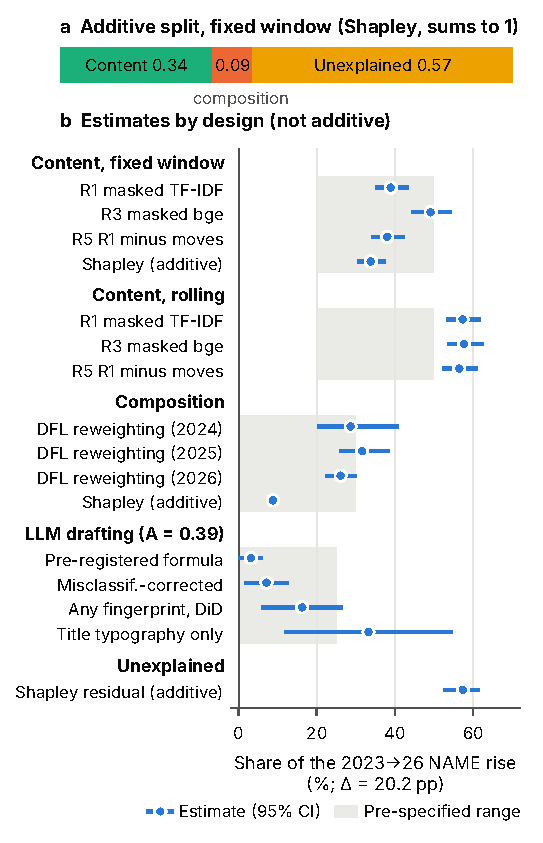
\includegraphics[width=\columnwidth]{fig2_decomposition.pdf}
\caption{\textbf{What accounts for the 2023$\rightarrow$26 \NAME{} rise} ($\Delta=20.2$\pp). (a) The one additive split (fixed-window Shapley). (b) Estimates from separate designs, which are \emph{not} additive: name-masked content (fixed and rolling), composition (DFL for each of 2024--26; Shapley), detectable LLM drafting under four estimators at an adoption rate of 0.39, and the Shapley residual. Grey bands: pre-specified predictions. CIs: conditional paper bootstrap ($B=2000$); tool-share CIs propagate the CI of the fingerprint uplift.}
\label{fig:nt-decomp}
\end{figure}

\subsection{Who carries it}
\label{sec:nt-carriers}

\paragraph{The pooled ratio is not diagnostic.}
At the last list position, papers carrying a stayer key moved from 18.8\% to 37.1\% \NAME{} between E and L, almost exactly the population's 19.4\% to 37.8\% (stayer ratio $\rho_{\text{last}}=0.995$ \ci{0.943}{1.050}). This looks like communal change, but a title is shared by every co-author: in L, 69\% of papers with a stayer key at the last position (7,889 of 11,503) have an entrant key at the first position. A purely generational world, in which only papers with an entrant key at the first position changed, combined with the observed co-authorship, gives $\rho_{\text{last}}$ of 0.88--0.93 and $\rho_{\text{any}}$ of 0.78--0.82, above the pre-specified thresholds. The prediction is met, but communal change is \textbf{not identified}. Our first caution: key-level within-incumbent shares of co-authored text need a shared-outcome generational null.

\paragraph{The rise is graded by team newness} (Figure~\ref{fig:nt-carriers}a).
Relative to the population change (18.3\pp), papers whose keys are all stayers changed 0.06 \ci{-0.14}{0.28} times as much, and papers whose keys were all present in 2021--22 $-0.07$ \ci{-0.42}{0.24} times (this fixed-base row has E $=$ 2023 and is a ratio to that window's 17.5\pp). Last-position stayer keys on papers without an entrant co-author key changed 0.22 \ci{0.07}{0.37} times as much, teams whose keys were all seen the year before 0.70 \ci{0.49}{0.90}, and last-position stayer keys on papers with an entrant first-position key 1.14 \ci{1.07}{1.20}. A pre-specified test (H2c) predicted that stayer keys' change, extrapolated in a key-fixed-effects regression to a zero share of new co-author keys, would be at least half the population change; it is 0.34 \ci{0.19}{0.48} times as much, so the prediction fails. H2c is a regression estimate at zero share of new co-authors, whereas the ``no entrant co-author'' row is a subgroup of L papers without any key first seen in L. Papers whose keys were all stayer keys barely moved, and among the 297 retitled resubmission pairs that survive the export (one submission per family, so pairs are selected on retitling) \NAME{} was not added on net (28 adds, 28 drops; mean 0.000, se 0.025). Whether this lags the content-fixed drift is not established ($-4.8$\pp{} against topic-adjusted drift, $p=0.057$). The style rides in with new projects and newcomer-containing teams. Groups of keys that did not adopt the style may also be the ones that did not add co-authors, and who chose a title on a mixed team is not identified.

\paragraph{First-position newcomer premium.}
In L, papers whose first-position key is an entrant carry \NAME{} titles 10.6\pp{} \ci{8.5}{12.6} more often than papers whose first-position key is a stayer; within the same last-position key, with team-size and topic fixed effects, the gap is 4.9\pp{} \ci{2.2}{7.6}. Stayers have at least three years of panel presence, so the contrast mixes cohort with tenure. With a symmetric two-year lookback the premium is absent in 2023 ($-0.2$\pp{} raw) and appears from 2024 (change to 2025--26: $+4.3$\pp{} \ci{0.3}{8.4}). This is a contrast between position labels, not a role effect.

\paragraph{Style versus topic.}
For 52 title-style and 33 abstract-topic markers we compute the generational increment $G$. Within-stayer change keeps pace with topic markers ($G_{\text{topic}}=-0.05$ \ci{-0.07}{-0.03}) but lags style markers ($G_{\text{style}}=0.17$ \ci{0.13}{0.20}) (Figure~\ref{fig:nt-carriers}b). A shared-outcome null predicts the same ratio for every marker, so a difference between channels cannot come from co-authorship composition. The weighted statistic is dominated by the \NAME{} family (93\% of the style weight) and the LLM-topic marker (94.5\% of the topic weight), but the contrast survives dropping both (difference 0.19 \ci{0.13}{0.26}) and equal marker weights (median per-marker ratio: style 0.84, topic 1.05). The gap sits at the first list position ($G_{\text{style}}=0.40$) and vanishes at the last (0.01). \textbf{Incumbent keys track topic shifts fully but style shifts only partly.}

\begin{figure*}[t]
\centering
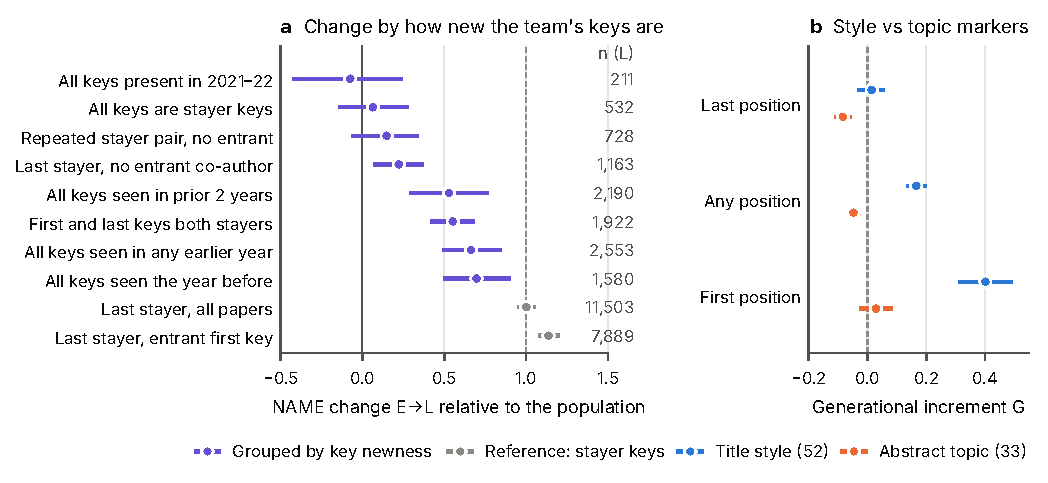
\includegraphics[width=0.84\textwidth]{fig3_carriers.pdf}
\caption{\textbf{Who carries the \NAME{} rise} (declared profile keys; list position is a label only). (a) \NAME{} change between E $=$ 2022--23 and L $=$ 2025--26 on papers grouped by how new their keys are, as a ratio of the paper-level population change (18.3\pp; 17.5\pp{} for the fixed-base 2021--22 row, whose early window is 2023; key-cluster bootstrap 95\% CIs; right column: L-period papers). The reference row ``Last stayer, all papers'' is a ratio to the paper-level change, not $\rho_{\text{last}}$. (b) Generational increment $G$ for 52 title-style and 33 abstract-topic markers by list position.}
\label{fig:nt-carriers}
\end{figure*}

\subsection{LLM-era wording in meaning-fixed slots}
\label{sec:nt-register}

\paragraph{Slots.}
Comparing synonyms that compete for the same opening slot holds what the title claims approximately fixed, conditional on a slot being filled. Among 1,922 slot-filled titles (2018--26), the LLM-favoured variant's share was 0.34 in 2023, 0.54 in 2024 and 0.67 in 2026 (Figure~\ref{fig:nt-register}a). In the pre-specified model with slot-specific trends, the 2024 level shift is OR 2.18 \ci{1.41}{3.38} for the slots and 0.87 \ci{0.64}{1.18} for the pooled controls, and the slot-minus-control contrast is 2.55 \ci{1.53}{4.25} (Holm $p<0.001$). It holds in the camera-ready-free pool (2.18 \ci{1.28}{3.70}) and the non-LLM subset (2.59 \ci{1.57}{4.28}). Per 1,000 titles, LLM-variant openers rose from 11.4 (2023) to 30.0 (2024) while neutral variants stayed flat (22.0 to 25.2): level shifts RR 3.91 \ci{1.84}{8.29} against 1.17 \ci{0.70}{1.94}. In 2024 the new verbs were \emph{added} rather than swapped for their neutral synonyms; substitution appears only in 2025--26.

\paragraph{Qualifications.}
(i) The pooled control null rests on via/using, 76\% of control titles and itself LLM-associated \citep{geng2026beyond}. Fitted alone, towards/toward (1.69 \ci{0.82}{3.47}) and novel/new (1.58 \ci{0.74}{3.36}) sit above the pre-specified 1.5 bound; the pooled controls shift significantly at every other candidate break year and under a level contrast (2.02 \ci{1.73}{2.37}); and without via/using the slot-minus-control contrast is 1.41 \ci{0.74}{2.68}. The pooled control share itself rose from 0.72 (2023) to 0.87 (2026), mostly via/using (Figure~\ref{fig:nt-register}a). (ii) The OR $\geq 2$ margin depends on \emph{enhancing}, chosen after the pilot saw it in these titles; without it the slot OR is 1.72 \ci{1.04}{2.84}. (iii) Part of the rise may begin with the 2023 cohort, submitted before ChatGPT's release (slot OR 2.2--2.4; CIs include 1). (iv) The audit cannot check slot words (23 accepted / 5 rejected v1 titles carry them).

\paragraph{Word families.}
2024 LLM title words fell from 63.1 to 47.8 per 1,000 titles between 2025 and 2026 while 2026 LLM title words rose from 23.3 to 46.4 (Figure~\ref{fig:nt-register}b), but their neutral synonyms fell alike, so this is a shift in word families, not an identified register turnover (Appendix~\ref{app:nt-more}).

\paragraph{Lexical and structural associations.}
Abstract LLM fingerprints go with both the lexical choice (LLM slot variant, OR 1.42 \ci{1.14}{1.79}) and branding (\NAME{} in the population, OR 1.14 \ci{1.08}{1.21}). The lexical association is not detectably larger: the ratio is 1.24 \ci{0.99}{1.57} (one-sided $p=0.030$), 1.19 \ci{0.84}{1.65} with the strict fingerprint, and 0.99 \ci{0.71}{1.45} in 2026 (Figure~\ref{fig:nt-register}c), so the pre-specified $1.5\times$ is not met. The pre-specified same-paper comparator (1.55) is \textbf{collider-conditioned}: slot filling is a common effect of the fingerprint and of \NAME{} (a \NAME{} title moves the slot to the subtitle), with a selection factor of 0.79. This is our second caution. Whether the wording also appears on papers without a detectable fingerprint stays unresolved ($U^*=0.65$ \ci{0.50}{0.81}, below the pre-specified 0.8).

\begin{figure*}[t]
\centering
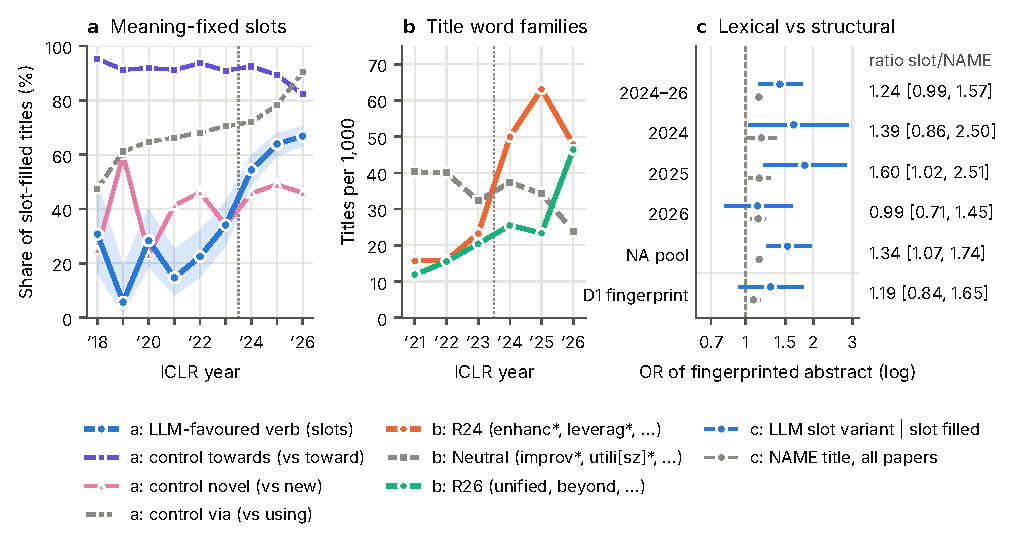
\includegraphics[width=0.92\textwidth]{fig4_register.pdf}
\caption{\textbf{LLM-favoured wording in titles} (associational). (a) Share of slot-filled titles that use the LLM-favoured verb (\emph{Enhancing/Boosting} vs \emph{Improving}; \emph{Unveiling} vs \emph{Understanding}; \emph{Leveraging} vs \emph{Exploiting}; \emph{comprehensive} vs \emph{systematic}; 95\% Wilson band), and the share of the first variant in each control pair, shown separately; via/using (dashed) carries 76\% of control titles and drifts upward, which is why the pooled control null holds only at the 2024 specification. (b) Title rates per 1,000 of the 2024 LLM title words, their neutral synonyms and the 2026 LLM title words. (c) Association of the abstract LLM-word fingerprint (F\_any) with the LLM slot variant (slot-filled papers) and with \NAME{} (all papers), within topic100 $\times$ year; right column: ratio OR$_{\text{slot}}$/OR$_{\text{NAME}}$, including 0.99 in 2026. ``D1 fingerprint'' is the strict F\_d1, with which the positive control is not significant.}
\label{fig:nt-register}
\end{figure*}

\subsection{Review selection and published-only bias}
\label{sec:nt-review}

\paragraph{Stage gains.}
For 2024--26 we decompose the accepted/all ratio of each feature into a desk stage, an author-exit stage (withdrawal before the decision) and a decision stage (Appendix Figure~\ref{fig:nt-gains}, Table~\ref{tab:filter}). For \NAME{}, the exit gain is 0.974 \ci{0.965}{0.983} and the decision gain 1.050 \ci{1.028}{1.072}; they net to a total of 1.021 (90\% CI \ci{1.001}{1.041}). With topic, area and team-size adjustment the stage gains are indistinguishable from 1 (exit 0.993, decision 1.019). The pre-specified equivalence test passes (TOST in \ci{0.90}{1.11}) and survives the camera-ready audit: the editing-corrected 90\% CI is \ci{0.949}{1.031}. The slope change does not differ detectably between the accepted, rejected and withdrawn pools (ORs 1.05 / 1.12 / 1.11, ITS 2018--26; equality $p=0.51$), though equivalence is not shown.

The decision-stage enrichment itself is not identified: the \NAME{} net-flip DiD is $+1.48$\pp{} \ci{-0.63}{3.59} against a tipping point of 2.92\pp. At the audit's point estimate about half of the stored-title \NAME{} excess among accepted papers would be attributable to camera-ready editing, but the CI ($-21\%$ to 124\%) spans both no editing effect and more than the whole association. \textbf{No title feature's acceptance association passes the Holm-controlled gate (0 of 18 auditable)}; an uncorrected rule would have passed compound titles and outsider casing without ALL-CAPS. \textbf{The published record is neutral for \NAME{} titles}: accepted papers carry them at the all-submission rate, also after correcting for camera-ready edits, while whether the decision stage itself adds a small premium cannot be told apart from camera-ready renaming. Stage gains measure selection on observed titles; whether authors brand in anticipation of reviewer taste is outside this design.


\paragraph{LLM markers.}
There is no evidence that decisions select against LLM-styled titles or abstracts as such. The LLM-style union is 0.975 \ci{0.951}{1.001} in total, which fails Holm. Its depletion is carried by 2024 LLM title words (``Enhancing X via Y''), which were depleted at the withdrawal stage at a similar rate before 2024 (exit OR 0.723 in 2018--23 vs 0.740 in 2024--26); their observed decision-stage gain (0.896) is not identified against editing. Without them the union is neutral (0.998 \ci{0.972}{1.027}). One pattern is new: the camera-ready-free pre-decision gain is 0.965 \ci{0.939}{0.993} for F24 abstracts and 0.963 \ci{0.957}{0.970} for the abstract style density, a 3--4\% depletion located before the decision (desk rejection and withdrawal). No decision-stage association of these markers is identified against editing, so the decision stage is not shown to be neutral either. The F24 part is new only against a baseline that includes 2023 (post/pre 0.914 \ci{0.849}{0.988} vs 2018--23; 0.975 \ci{0.893}{1.071} vs 2018--22). Before 2024 the LLM-style union was \emph{enriched} among accepted papers (1.154 \ci{1.070}{1.236}).

\paragraph{What a published-only study would see.}
Comparing accepted-only with all-submission statistics (Appendix Figure~\ref{fig:nt-bias}a), 9 of 11 mainstream statistics fall within $\pm 10\%$ (\NAME{} 1.021), against 1 of 4 outsider and 7 of 9 LLM-style statistics. ALL-CAPS titles appear at 0.36 \ci{0.26}{0.47} of their all-submission share, and 2024 LLM title words at 0.807 \ci{0.740}{0.874}. For the 2024 \NAME{} slope change the effect-scale ratio is 0.50 \ci{-0.15}{1.16}: a published-only study's estimate of the acceleration is about half as large, but the interval includes full recovery. In the accepted pool alone the slope change is not detected (OR 1.053, $p=0.18$; ITS 2018--26), and the colon-premium trend ratio is 0.89 (0.66--1.12).

\paragraph{Kobak-style bounds.}
For abstracts, accepted-only excess-vocabulary bounds of LLM use fall below all-submission bounds in each year (ratios 0.80, 0.71 and 0.50 for 2024--26), but the pre-specified $\geq 15\%$ understatement is not established in any year, and the yearly fall of the bounds reflects vocabulary decay, not a fall in LLM use (Appendix~\ref{app:nt-more}).

\paragraph{Withdrawals.}
The raw withdrawal excess of \NAME{} papers is mostly topic composition (Appendix~\ref{app:nt-more}).

